% \usepackage{graphicx}; \graphicspath{{<path to this folder>/}}

\begin{figure}[htbp]
  \centering
  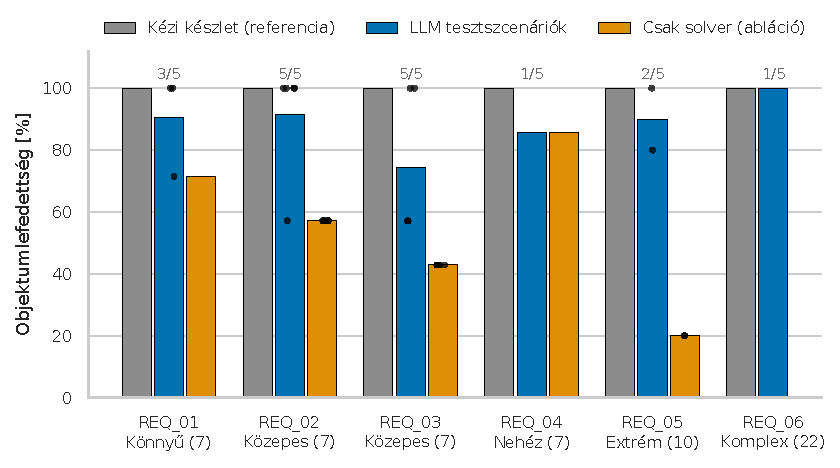
\includegraphics[width=\textwidth]{fig1_coverage_per_requirement}
  \caption{Követelményenkénti objektumlefedettség a kézi referencia-készlet, az LLM által tervezett tesztszcenáriók és a csak solveres abláció (generált megszorítások szcenáriók nélkül) esetén. Oszlop: a sikeres futások átlaga; pont: egyes futások; a csoportok fölött: sikeres/összes futás; zárójelben: a lefedettségi elemek száma.}
  \label{fig:fig1-coverage-per-requirement}
\end{figure}

\begin{figure}[htbp]
  \centering
  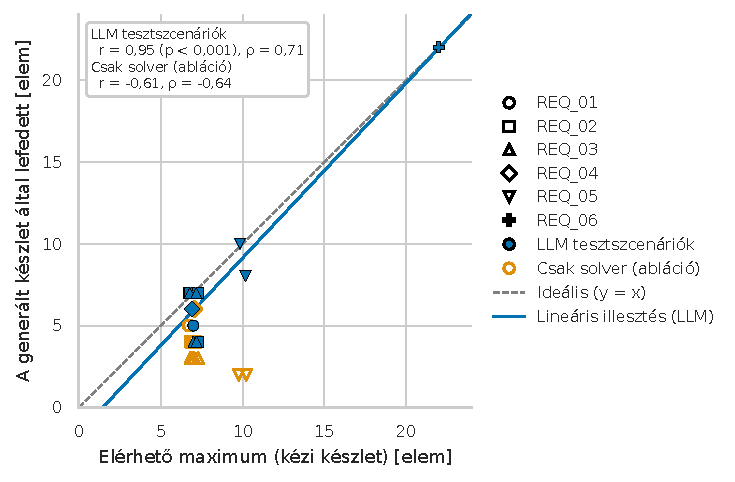
\includegraphics[width=0.85\textwidth]{fig2_correlation}
  \caption{A generált készletek által lefedett elemek száma a kézi készlettel meghatározott elérhető maximum függvényében. Minden pont egy sikeres futás; a szaggatott vonal a tökéletes egyezés.}
  \label{fig:fig2-correlation}
\end{figure}

\begin{figure}[htbp]
  \centering
  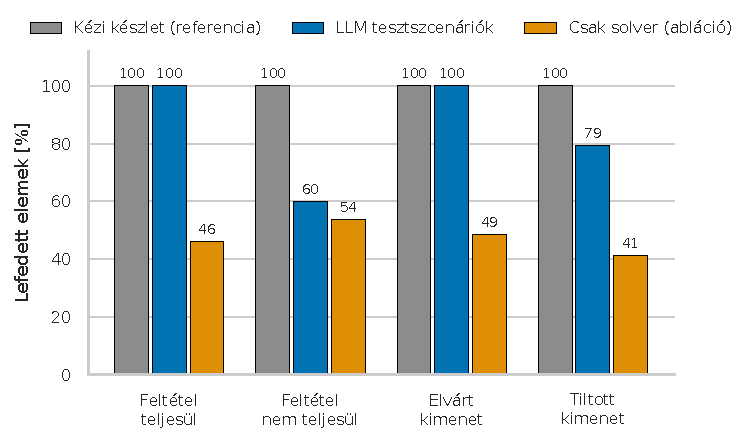
\includegraphics[width=0.85\textwidth]{fig3_item_categories}
  \caption{Lefedettség elemkategóriánként (feltétel teljesül, feltétel nem teljesül, elvárt kimenet, tiltott kimenet), az összes követelményre és sikeres futásra összesítve.}
  \label{fig:fig3-item-categories}
\end{figure}

\begin{figure}[htbp]
  \centering
  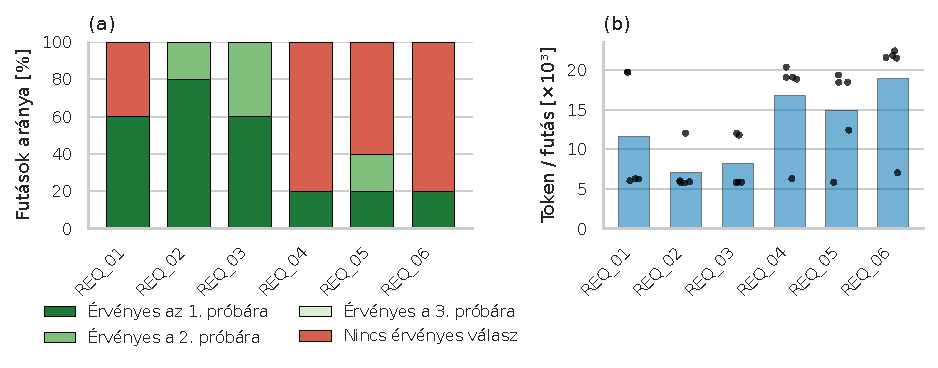
\includegraphics[width=\textwidth]{fig4_reliability_and_cost}
  \caption{(a) A futások kimenete: hányadik próbálkozásra fogadta el a Refinery az LLM válaszát, illetve az utolsó javítási kör után sincs érvényes válasz. (b) Futásonként felhasznált tokenek, az összes javítási körre összegezve.}
  \label{fig:fig4-reliability-and-cost}
\end{figure}

\begin{figure}[htbp]
  \centering
  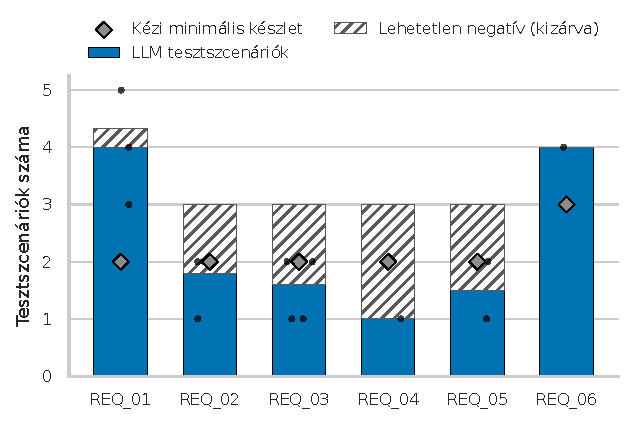
\includegraphics[width=0.75\textwidth]{fig5_suite_size}
  \caption{Az LLM által tervezett tesztszcenáriók száma készletenként, a kézi minimális készlettel összevetve. Sraffozva: a negatív esetként megjelölt szcenáriók, amelyek már a rendszermodellben (a generált megszorítások nélkül) kielégíthetetlenek; ezek kikerültek a készletből, és a lefedettségbe nem számítanak bele.}
  \label{fig:fig5-suite-size}
\end{figure}

\begin{figure}[htbp]
  \centering
  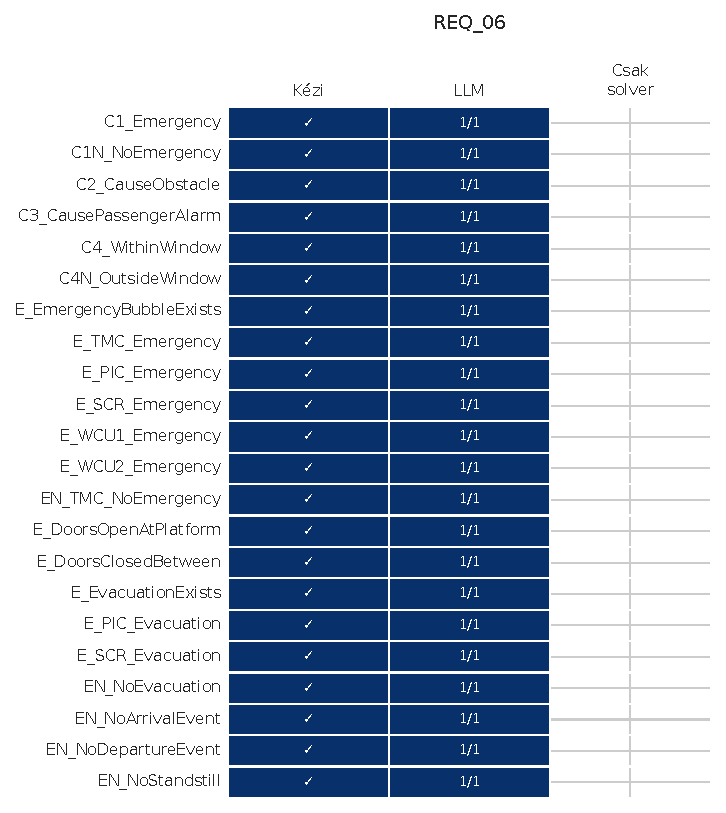
\includegraphics[width=0.6\textwidth]{fig6_items_REQ_06}
  \caption{REQ_06 lefedettségi elemei: a kézi készlet, valamint azon sikeres futások aránya, amelyekben a generált készlet (és a csak solveres abláció) tanúsította az elemet.}
  \label{fig:fig6-items-REQ-06}
\end{figure}
